
\marginpar{\href{https://youtu.be/l4NoMKEHQwM}{Video}}
\marginpar{\href{https://ocw.mit.edu/courses/6-041sc-probabilistic-systems-analysis-and-applied-probability-fall-2013/pages/unit-ii/lecture-11/}{Lecture Home}}
\marginpar{\href{https://ocw.mit.edu/courses/6-041sc-probabilistic-systems-analysis-and-applied-probability-fall-2013/e4eb782ee3db745a86a3cef03d4c9e30_MIT6_041SCF13_L11.pdf}{Slides}}
Reading: 4.1, 4.2

How to derive the distribution of a function of a random variable.

$W=X+Y$ - shows up often

\begin{figure}[h]
\centering
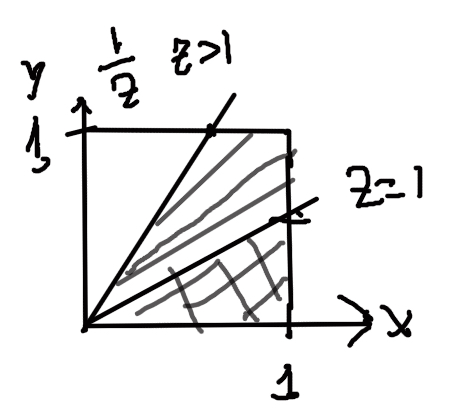
\includegraphics[width=5cm, height=4cm]{images/L11/derived_dist_z.jpeg}
\caption{$Z=g(X,Y)=\frac{Y}{X}$}
\end{figure}

Find PDF of $Z=g(X,Y)=\frac{Y}{X}$

\begin{align*}
F_z{z}=P \left(\frac{Y}{X} \le Z \right) = \frac{Z}{2},\quad Z le 1
\end{align*}

\begin{align*}
F_z{z}= 1 - \frac{1}{2}1\frac{1}{Z} = \frac{1}{2},\quad Z \ge 1\\
F_z{z}= 0, Z < 0
\end{align*}

\begin{align*}
E[Z] = \int_0^1 z \frac{1}{2}dz + \int_1^{\infty} \underbrace{z \frac{1}{2 z^2}dz}_{\infty}
\end{align*}
We get an infinite expectation.  That's nothing strange.

\marginpar{(13:25)}

A general formula: -don't need to go through cumulative.


Let $Y=g(X)$, g strictly monotonic

\marginpar{(18:20)}

$Y=X^3$, $g(X)=X^3 = y$
$X=y^\frac{1}{3}$

\begin{align*}
f_X(x)=f_{Y}(y)\cdot 3x^2
f_Y(y)=?
 = f_X(y^\frac{1}{3}) \cdot \frac{1}{3y^\frac{2}{3}}
\end{align*}

\marginpar{20:30)}

\begin{figure}[h]
\centering
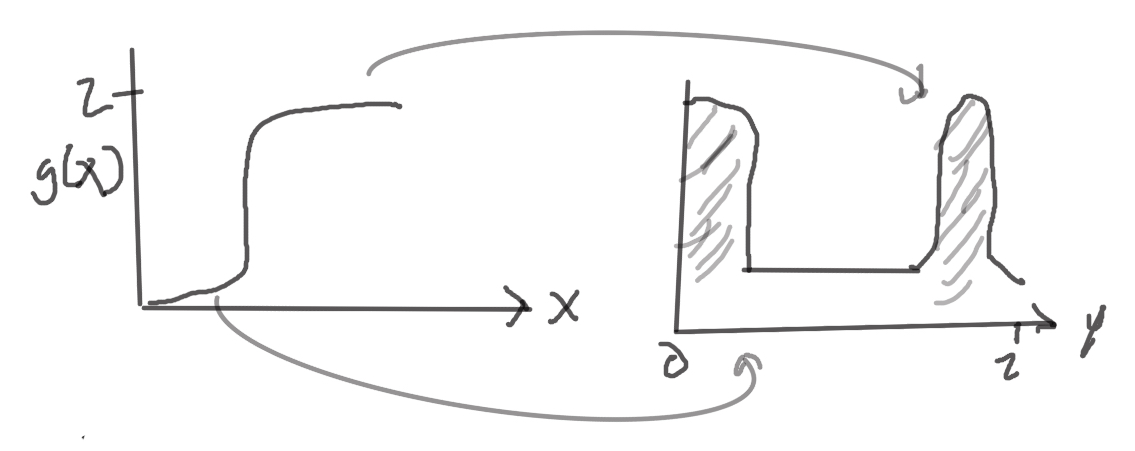
\includegraphics[width=6cm, height=4cm]{images/L11/strictly_monotonic.jpeg}
\caption{x}
\end{figure}

NOTE: y tales values close to zero. Flat $g()$ gives more density.

\subsection{Distribution of X+Y}

\marginpar{24:30)}

\begin{figure}[h]
\centering
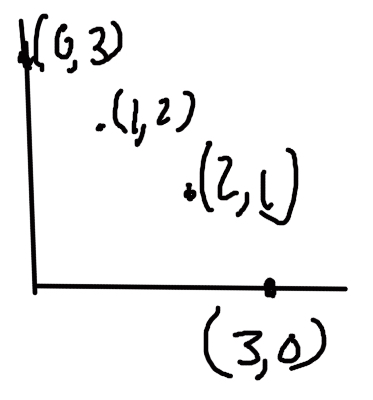
\includegraphics[width=6cm, height=4cm]{images/L11/dist_x_y.jpeg}
\caption{x}
\end{figure}

\subsection{Continuous Case}

\marginpar{31:50)}

Slide.

See derivation in text.

\subsection{Two Independent Normal RVs}

\marginpar{33:30)}

\begin{itemize}
    \item What does joint PDF look like?
    \item Ellipses, centered at $\mu_x, \mu_y$
\end{itemize}

\begin{figure}[h]
\centering
\begin{minipage}{.45\linewidth}
  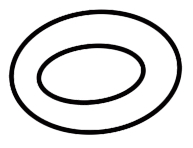
\includegraphics[width=\linewidth]{images/L11/wider.jpeg}
  \caption{$\sigma_x > \sigma_y$}
  \label{wider}
\end{minipage}
\hspace{.05\linewidth}
\begin{minipage}{.45\linewidth}
  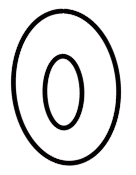
\includegraphics[width=\linewidth]{images/L11/taller.jpeg}
  \caption{$\sigma_x < \sigma_y$}
  \label{taller}
\end{minipage}
\end{figure}

\begin{figure}[h]
\centering
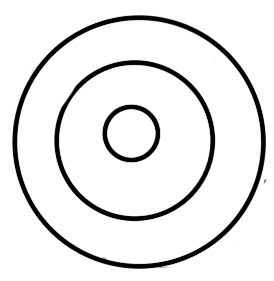
\includegraphics[width=6cm, height=4cm]{images/L11/percent_circle.jpeg}
\caption{$\sigma_x = \sigma_y$}
\end{figure}

\subsection{Sum of Independent Normal Random Variables}

\marginpar{39:20)}

$X \sim N(0, \sigma_x^2), \qquad Y \sim N(0, \sigma_y^2)$

Let $W=X+Y$.  The sum is also normal: $mean=0,var=\sigma_x^2 + \sigma_y^2$

\subsection{Covariance}

\marginpar{41:40)}

\begin{align}
    cov(X,Y)=E[X-E[X]] - [Y - E[Y]] \\
    = E[XY] - E[X]E[Y]
\end{align}
\myequations{Covariance}

\begin{align*}
cov(X,X)=var(X)
\end{align*}

Covariance has the wrong units.

\subsection{Correlation Coefficient}

\marginpar{48m)}

\begin{align}
\rho = \frac{cov(X,Y)}{\sigma_X \sigma_Y}, \qquad 0 \le \rho \le 1
\end{align}
\myequations{Correlation Coefficient}

Removes units

$\rho$ is the correlation coefficient.